\documentclass[12pt]{article}
\usepackage[margin=1in]{geometry}  
\usepackage{amsmath, amsthm, amssymb, amsfonts, enumitem, fancyhdr, color, comment, graphicx, environ, tipa, multicol, array, xparse, xcolor, qtree, lastpage, listings, hyperref, bookmark, apacite, lipsum, algorithm}
\pagestyle{fancy}
\bibliographystyle{apacite}

% commands 
\newcommand{\la}{$\leftarrow $}
\newcommand{\ra}{$\rightarrow $ }
\newcommand\todo[1]{\textcolor{red}{(#1)}}
\newcounter{equationset}
\newcommand{\equationset}[1]{% \equationset{<caption>}
  \refstepcounter{equationset}% Step counter
  \noindent\makebox[\linewidth]{Equation~\theequationset: #1}}% Print caption



 


\setlength{\headheight}{45pt}
\cfoot{}
\lstset{%for listing /code 
  basicstyle=\ttfamily,
  columns=fullflexible,
  frame=single,
  breaklines=true,
  postbreak=\mbox{\textcolor{red}{$\hookrightarrow$}\space},
}
%%%%%%%%%%%%%%%%%%%%%%%%%%%%%%%%%%%%%%%%%%%%%%%%%%%%%
\lhead{Lawrence Fulton - 433218} 
\rhead{ \thepage \space of \pageref{LastPage}} 


\newcommand{\researchquestion}[1]{\begin{quote}\sloppy \emph{#1} \end{quote}} 



\title{Description of Planned Statistics for the Project}
\author{Lawrence Fulton (\url{lawrence.fulton@rwth-aachen.de})\\ Computational Social Systems -  RWTH Aachen}


%%%%%%%%%%%%%%%%%%%%%%%%%%%%%%%%%%%%%%%%%%%%%
\begin{document}
\maketitle


\section{Prompt Sensitivity}
\subsection{Prompt Generation}
For the later research it is important to understand how sensitive the model is with regards to the prompt. For this we will run the experiment with different prompts and then compare the results. The prompts will be created the following, where the content inside the square brackets is the type of prompt, indicating if it is either "system", "user", or "assistant". There are always two different versions per prompt, one for the LLM to generate a new reply for the debate and one for it to generate a value how much the LLM agrees to the statements.
The content inside the curly brackets is a placeholder for the actual content that will be inserted later and will be the same for all prompts. The \{user\_answer\} and \{assistant\_answer\} will be the previous replies of the user and the assistant.

\begin{table}[h!]
\caption{Overview of Variables for Prompt Sensitivity Experiment}

\begin{tabular}{|l|l|}
\hline
Variable             & Example                                                                                                                                                                                                                                                                                                                                                                                                                                                                                                                                                                                      \\ \hline
experiment\_scenario & \begin{tabular}[c]{@{}l@{}}Du diskutierst über die Aussage: Die Förderung von Windenergie \\ soll beendet werden.\end{tabular}                                                                                                                                                                                                                                                                                                                                                                                                                                                               \\ \hline
background\_story    & \begin{tabular}[c]{@{}l@{}}Ich bin 75 Jahre alt und männlich. Ich habe einen Hauptschulabschluss, \\ ein mittleres monatliches Haushalts-Nettoeinkommen und ich bin nicht \\ berufstätig. Ich bin etwas religiös. Politisch-ideologisch ordne ich mich \\ in der Mitte ein. Ich identifiziere mich mäßig mit der Partei SPD und \\ habe SPD gewählt. Ich lebe in Westdeutschland. Ich finde, die Regierung \\ sollte die Einwanderung einschränken und habe keine Meinung dazu, \\ ob die Regierung Maßnahmen ergreifen sollte, um die \\ Einkommensunterschiede zu verringern.\end{tabular} \\ \hline
question\_prompt     & \begin{tabular}[c]{@{}l@{}}Auf einer Skala von 1 bis 7: Wie sehr stimmst du der Aussage zu: \\ Die Förderung von Windenergie soll beendet werden. Antworte nur \\ mit einer Zahl.\end{tabular}                                                                                                                                                                                                                                                                                                                                                                                               \\ \hline
\end{tabular}
\label{tab:variables_prompt_sensitivity}
\end{table}

% code section

\begin{lstlisting}[caption={Prompt 1 - Discussion Prompt}]
[System] Scenario: {experiment_scenario}
Background Story: {background_story}
The following is a a debate between you and another person.
[User] {user_answer}
[Assistant] {assistant_answer}
[User] {user_answer_2}
{...}
\end{lstlisting}
In case we are prompting the model to generate the answer we will use the following prompt:
\begin{lstlisting}[caption={Prompt 1 - Answer Generation}]
[System] Scenario: {experiment_scenario}
Background Story: {background_story}
The following is a debate between you and and another person. Complete your next reply. Keep the reply shorter than 30 words and in German. 
[User] {user_answer}
[Assistant] {assistant_answer}
[User] {user_answer_2}
[Assistant] {assistant_answer_2}
{...}
[User] {question_prompt}
\end{lstlisting}


The second prompt will be more expressive:


\begin{lstlisting}[caption={Prompt 2 - Discussion Prompt}]
[System] The scenario is the following: {experiment_scenario}
This is your background story: {background_story}
The following is a conversation between you and another person. Complete your next reply. Keep the reply shorter than 30 words and in German.
[User] {user_answer}
[Assistant] {assistant_answer}
[User] {user_answer_2}
{...}
\end{lstlisting}
In case we are prompting the model to generate the answer we will use the following prompt:
\begin{lstlisting}[caption={Prompt 2 - Answer Generation}]
[System] The scenario is the following: {experiment_scenario}
This is your background story: {background_story}
The following is a conversation between you and another person.
[User] {user_answer}
[Assistant] {assistant_answer}  
[User] {user_answer_2}
[Assistant] {assistant_answer_2}
{...}    
User: {question_prompt} 
\end{lstlisting}




The third prompt version adds some additional new lines and rewords the instructions slightly:
\begin{lstlisting}[caption={Prompt 3 - Discussion Prompt}]
[System] Scenario: {experiment_scenario}
Background Story: {background_story}
You are about to have a conversation with another person.
Respond to the next message. Please keep your reply under 30 words and in German.
[User] {user_answer}
[Assistant] {assistant_answer}
[User] {user_answer_2}
{...}
\end{lstlisting}    

In case we are prompting the model to generate the answer we will use the following prompt:
\begin{lstlisting}[caption={Prompt 3 - Answer Generation}]
[System] Scenario: {experiment_scenario}
Background Story: {background_story}
You are about to have a conversation with another person.
Please reply with only a number.
[User] {user_answer}
[Assistant] {assistant_answer}
[User] {user_answer_2}
[Assistant] {assistant_answer_2}
[...]
[User] {question_prompt}
\end{lstlisting}


\subsection{Prompt Sensitivity Analysis}
\subsubsection{Visualisation}
To analyse the sensitivity of the model to the different prompts we will run the experiment with each prompt and then compare the results. Since we have seven parties (Die Linke, SPD, Bündnis 90/Die Grünen, FDP, CDU/CSU, AfD, default) and we are testing all parties with all parties this will lead to a total of  $\sum_{i=1}^{7} i = 28$ different combinations of parties. For each combination we will run the experiment with each of the three prompts, leading to a total of $28 \times 3 = 84$ experiments. Each experiment will be repeated 5 times which results in a total of $84 \times 5 = 420$ experiments per question. For now I am only applying it to one question but this is easily extendable to all questions. We prompt the LLM to generate us the answer to the \{question\_prompt\} at every 4th step of the discussion. The LLM will then generate a number between 1 and 7, which is the answer to the question. We will then compare the answers of the LLM for each party and each prompt.

To get a graphical overview over the spread of the results per prompt we have normalised the data for each party at each discussion step. This is done since we expect that members of different parties will have very different opinion to the topics given and this would allow us to compare the all of the results. The method used for the normalisation is the Standard Scaler from the sklearn library. The Standard Scaler normalises the data by subtracting the mean and dividing by the standard deviation. This results in a distribution with a mean of 0 and a standard deviation of 1. The results can be seen in the following: 

\begin{figure}[h!]
\centering
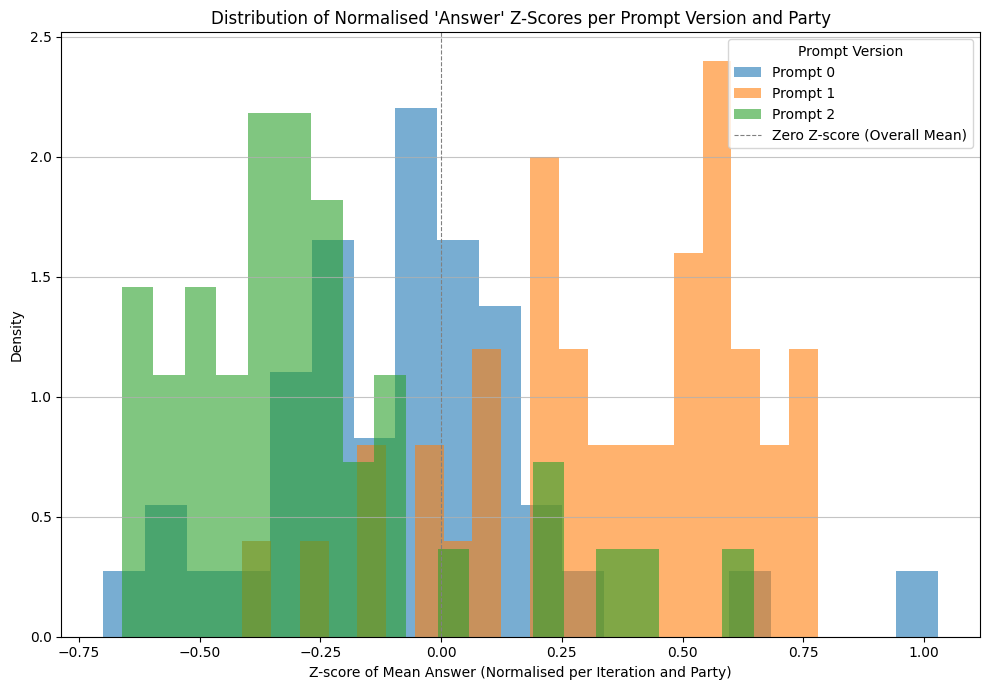
\includegraphics[width=0.8\textwidth]{img/normalised_results.png}
\caption{Histogram of the normalised results per each party and prompt. The x-axis shows the normalised values and the y-axis shows the frequency of these values. The different colors represent the different prompts used.}
\label{fig:normalised_results}
\end{figure}


\subsubsection{Statistical Analysis}

To analyse the statistical significance of the differences between the prompts we will use a mixed-effects model. The mixed-effects model allows us to account for the fact that we have repeated measures from the same debate sessions. We will use the `statsmodels` library in Python to fit the model.

In a mixed-effects model, we distinguish between fixed and random effects.
\begin{itemize}
    \item \textbf{Fixed Effects} are the variables we want to investigate directly. Our fixed effects are `version` (the prompt version), `party`, `time`, and `question\_index`, excluding their interactions. This allows us to test whether the prompt `version` has a significant effect on the `answer`, and how this effect might change depending on the party or over time.
    \item \textbf{Random Effects} account for sources of non-independent variance in the data. In this experiment, multiple answers are generated within the same debate. To account for this clustering, we will include a random intercept for each unique debate session. A debate session is uniquely identified by the combination of the parties debating, the prompt version, and the repetition number.
\end{itemize}

The model will have the following structure:
\begin{equation}
    \text{answer} \sim \text{version} + \text{party} + \text{time} + \text{question\_index} + (1 | \text{debate\_id})
\end{equation}
where `debate\_id` is a unique identifier for each experimental run. This model structure allows us to test our hypotheses about the prompts while correctly controlling for the nested structure of the data.

\subsection{Results}
The results of the mixed-effects model are presented in Table \ref{tab:mixed_model_results}. The analysis reveals a statistically significant effect of the prompt `version` on the `answer` provided by the model.

\begin{table}[h!]
\centering
\caption{Mixed-Effects Model Regression Results for `answer`}
\label{tab:mixed_model_results}
\begin{tabular}{lrrrr}
\hline
\textbf{Effect} & \textbf{Coef.} & \textbf{Std.Err.} & \textbf{z} & \textbf{$P>|z|$} \\
\hline
Intercept                       & 1.455    & 0.066  & 22.076 & \textless 0.001 \\
party[T.AfD]                    & 2.106    & 0.081  & 26.128 & \textless 0.001 \\
party[T.Bündnis 90/Die Grünen]  & 0.444    & 0.081  & 5.512  & \textless 0.001 \\
party[T.CDU/CSU]                & 0.663    & 0.081  & 8.224  & \textless 0.001 \\
party[T.Die Linke]              & 0.028    & 0.081  & 0.352  & 0.725 \\
party[T.FDP]                    & 0.133    & 0.081  & 1.652  & 0.099 \\
party[T.SPD]                    & 0.361    & 0.081  & 4.483  & \textless 0.001 \\
version[T.out\_1]                & 0.297    & 0.053  & 5.634  & \textless 0.001 \\
version[T.out\_2]               & -0.132   & 0.053  & -2.503 & 0.012 \\
time                            & -0.158   & 0.005  & -30.385& \textless 0.001 \\
\hline
\multicolumn{5}{l}{\textit{Note:} Group Var = 0.280. The baseline for `version` is Prompt 1.}
\end{tabular}
\end{table}

The model indicates that the prompt version has a significant impact on the generated answers. Compared to the baseline (Prompt 1), `version[T.out\_1]` (Prompt 2) is associated with a significant increase in the answer value by 0.297 ($\beta = 0.297$, SE = 0.053, $z = 5.634$, $p < 0.001$). Conversely, `version[T.out\_2]` (Prompt 3) is associated with a significant decrease in the answer value by 0.132 ($\beta = -0.132$, SE = 0.053, $z = -2.503$, $p = 0.012$). These results confirm that even slight variations in prompt wording can lead to statistically significant differences in the model's output. As expected, the `party` and `time` variables were also highly significant predictors.

Thus we can conclude that the model is sensitive to the prompt variations, and this sensitivity can be statistically quantified using a mixed-effects model. The results suggest that the choice of prompt can significantly influence the model's responses, which is crucial for interpreting the outcomes of our experiments.


\section{Change of opinion over time}
Seeing that the prompt version has a significant effect on the `answer` generated by the model, we now have to take this into consideration when analyising the change of the opinions over time and are not able to just focus on one prompt as which would have been sufficient if the prompt had no effect.

The research question we are interested in is "Does discussion cause agents' opinions to significantly shift from their starting points and converge towards more uniform stances?". To answer this question we will have to analyse the change of the opinions over time with the focus on two different aspects: Firstly, the change of the opinions over time, quantified by calculating the distance of the opinions at each time step to the initial opinion. Secondly, the convergence of the opinions over time, quantified by calculating the variance of the opinions at each time step. These metrics are question agnostic, allowing us to compare the results across different questions and prompts.

\subsection{Distance to Initial Opinion}

To analyse the change of opinion over time, we will calculate the distance of the opinions at each time step to the initial opinion. This will allow us to see how much the opinions have changed over time. The distance is calculated as the absolute difference between the initial opinion for each agent in each debate and the opinion at each time step. Since we calculate the difference from the initial opinion, and the difference between a number and itself is 0 we will ignore timestep 0 for this analysis (though still added in the figure). A plot of the distance to the initial opinion over time can be seen in Figure \ref{fig:distance_to_initial_opinion}.

\begin{figure}[h]
\centering
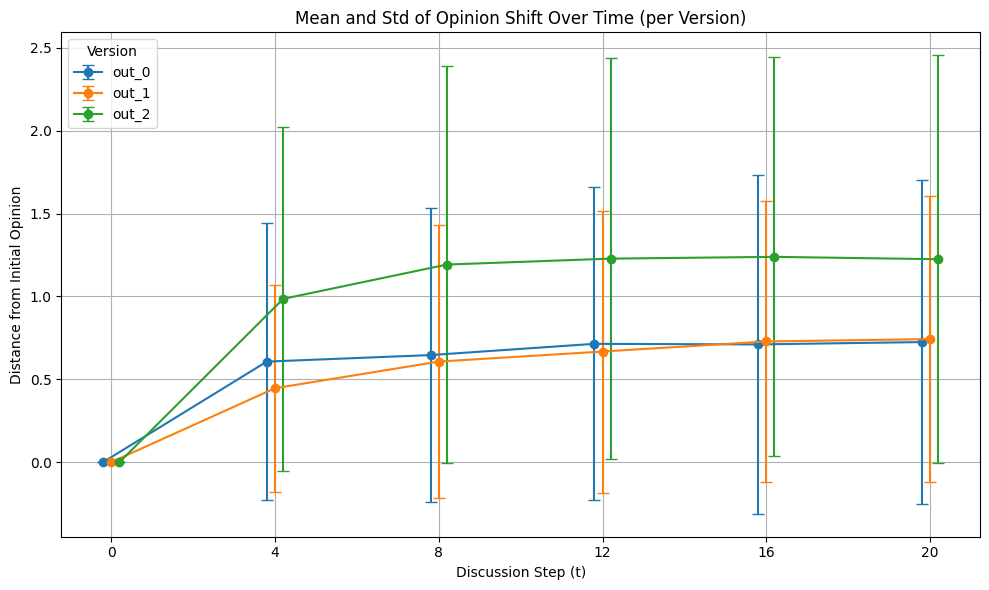
\includegraphics[width=0.8\textwidth]{img/distance_to_initial_opinion.png}
\caption{Distance to Initial Opinion Over Time}
\label{fig:distance_to_initial_opinion}
\end{figure}

We again use the mixed-effects model to analyse the change of opinion over time. The model will have the following structure:
\begin{equation}
    \text{distance} \sim \text{party} + \text{time} + (1 | \text{debate\_id})
\end{equation}
where `distance` is the distance to the initial opinion, `party` is the party of the agent, and `time` is the time step with the same random effect structure as before. There is a significant effect of time onto the answer  ($\beta = 0.008$, SE = 0.003, $z = 0.008$, $p < 0.004$).

We withhold the variable `version` for now since the categorical value `version` is one-hot encoded. Thus by adding the variable the first version will be considered the baseline. The interactions between time:version thus only show the differences between the versions and the baseline version. Thus if we want to see if time is significant we have to subdivide the data into the different versions and then analyse the significance of time for each version separately. Applying another mixed-effect model on the reduced dataset with only data from one prompt version we will get three further results with all being significant (p=[0.01,\textless 0.001, \textless 0.001]) and positive effect sizes $\beta=[0.008,0.018,0.013]$. 

Thus we can conclude that the distance to the initial opinion is significantly affected by the time step, meaning that the opinions shift over time. Though the effect sizes are fairly small, indicating that the opinions do not change drastically over time. 


\subsection{Variance of Opinions}
To analyse the convergence of the opinions over time, we will calculate the variance of the opinions at each time step. This will allow us to see how much the opinions are converging towards a common stance. The variance is calculated as the average of the squared differences from the mean opinion at each time step. This reduces the dataset quite drastically since we now aggregate over time steps. A plot of the variance of the opinions over time can be seen in Figure \ref{fig:variance_of_opinions}. 


\begin{figure}[h]
\centering
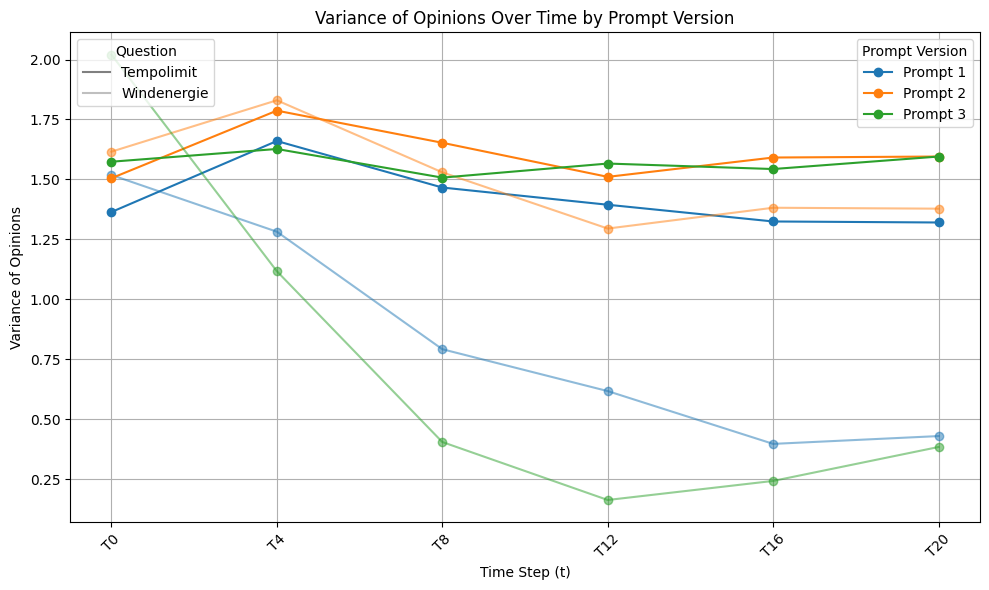
\includegraphics[width=0.8\textwidth]{img/variance_of_opinions.png}
\caption{Variance of Opinions Over Time}
\label{fig:variance_of_opinions}
\end{figure}

Since we are firstly interested in the convergence of the opinions over time we create the following mixed-effects model:
\begin{equation}
    \text{variance} \sim \text{time} + (1 | \text{prompt\_question})
\end{equation}
where `variance` is the variance of the opinions, and `time` is the time step. The prompt\_question now constitutes the random effect and consists out of a combination of the prompt version and the question index. Ideally this will give us a good overview over the convergence of the opinions over time. 

To understand if the variance is getting changing significantly over time we will again have to subdivide the data into the different prompt versions and then analyse the significance of time for each version separately. For this we will be fitting a simple linear mixed model for each with a subset of the data from each prompt version separately as seen in the following:
\begin{equation}
    \text{variance} \sim \text{time} + (1 | \text{question})
\end{equation}
where `variance` is the variance of the opinions, `time` is the time step, and `question` is the question index.ns.

\bibliography{ref}
\end{document}
